%This is a Latex file.
\documentclass[11pt]{article}
\usepackage{amsmath,amsfonts,amsthm}
\usepackage{dsfont}
\usepackage{fancyhdr}
\usepackage[margin=1in]{geometry}
\usepackage{lastpage} % Required to determine the last page for the footer
\usepackage{tikz}
\usepackage{url}

\theoremstyle{plain}
\theoremstyle{definition}
\newtheorem{exercise}{Exercise}

\pagestyle{fancy} 
\lhead{\sf Name} \chead{\sf HW \#X} \rhead{\sf Fall 2018 MTH 411} 
\lfoot{} \cfoot{\thepage} \rfoot{}

%% See Page 3 of Fraleigh
\newcommand{\C}{\mathbb{C}}
\newcommand{\R}{\mathbb{R}}
\newcommand{\Q}{\mathbb{Q}}
\newcommand{\Z}{\mathbb{Z}}

\newcommand{\Rplus}{\mathbb{R^+}}
\newcommand{\Qplus}{\mathbb{Q^+}}
\newcommand{\Zplus}{\mathbb{Z^+}}

\newcommand{\Cstar}{\mathbb{C^*}}
\newcommand{\Rstar}{\mathbb{R^*}}
\newcommand{\Qstar}{\mathbb{Q^*}}
\newcommand{\Zstar}{\mathbb{Z^*}}



\begin{document}

\begin{exercise} Prove that the summation identity \begin{equation}\label{Exercise1identity}1+4+9+\cdots+n^2 = \displaystyle\frac{n(n+1)(2n+1)}{6}\end{equation} holds for all $n \in \Zplus$.
\end{exercise}

\vspace{2ex}

\begin{proof}
In the case of $n = 1$, we have the left hand side of equation \eqref{Exercise1identity} is 1, while the right hand side is $\displaystyle\frac{1(2)(3)}{6} = 1$.  So equation \eqref{Exercise1identity} holds for $n = 1$.  
    
Suppose equation \eqref{Exercise1identity} holds for some $k \in \Zplus$.  We will now show that under this assumption, the identity holds for $k+1$.  We see that
    $$\begin{aligned}
    1 + 4 + 9 + \cdots + (k+1)^2 &= 1 + 4 + 9 + \cdots + k^2 + (k+1)^2\\
    &= \frac{k(k+1)(2k+1)}{6} + (k+1)^2, \text{ by assumption}\\
    &= (k+1)\left[\frac{k(2k+1)}{6} + (k+1)\right]\\
    &= (k+1)\left[\frac{k(2k+1)+6(k+1)}{6}\right]\\
    &= (k+1)\cdot\frac{2k^2+7k+6}{6}\\
    &= (k+1)\cdot\frac{(k+2)(2k+3)}{6}\\
    &= \frac{(k+1)(k+2)(2(k+1)+1)}{6}.
    \end{aligned}$$  Therefore, by the Principle of Mathematical Induction, equation \eqref{Exercise1identity} holds for all $n \in \Zplus$.
\end{proof}

\newpage

\begin{exercise}
Draw a Venn diagrams for $A\setminus B$ and $B\setminus A$.
\end{exercise}

\vspace{2ex}

\begin{center}
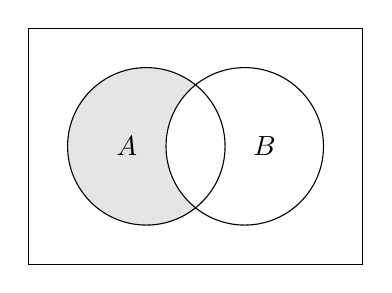
\begin{tikzpicture}
\draw (-1.5,-1.5) rectangle (2.75,1.5);
\begin{scope}
\fill[gray!20] (0,0) circle (1);    %draw grey circle first
\fill[white] (1.25,0) circle (1);
\end{scope}
\draw (0,0) circle (1);
\draw (1.25,0) circle (1);
	\draw (-.25,0) node {$A$};
	\draw (1.5,0) node {$B$};
	\end{tikzpicture}\\
	$A\setminus B$
\end{center}

\begin{center}
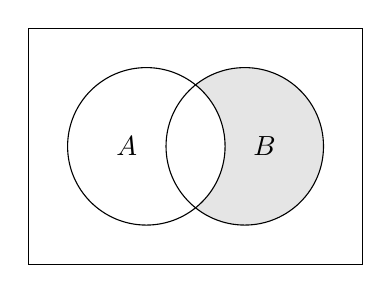
\begin{tikzpicture}
\draw (-1.5,-1.5) rectangle (2.75,1.5);
\begin{scope}
\fill[gray!20] (1.25,0) circle (1); %draw grey circle first
\fill[white] (0,0) circle (1);    
\end{scope}
\draw (0,0) circle (1);
\draw (1.25,0) circle (1);
\draw (-.25,0) node {$A$};
\draw (1.5,0) node {$B$};
\end{tikzpicture}\\
$B\setminus A$
\end{center}

\

\hrulefill

\

TikZ Resources:
\begin{itemize}
\item Jacques Cr\'emer, A very minimal introduction to TikZ:\\
\url{https://cremeronline.com/LaTeX/minimaltikz.pdf}
\item PGF and TikZ examples gallery:\\
\url{http://www.texample.net/tikz/examples/}
\item TeX - LaTeX Stack Exchange (covers all TeX related questions, not focused solely on TikZ):\\
\url{https://tex.stackexchange.com}
\end{itemize}


\end{document}
